\begin{frame}
\vfill
\centering
\begin{beamercolorbox}[sep=8pt,center,shadow=true,rounded=true]{title}
\usebeamerfont{title}Steering Behaviors
\end{beamercolorbox}
\vfill
\end{frame}

\begin{frame}{Anforderungen an Gegner}
\begin{itemize}
    \item Gegner sollen unterschiedliches Verhalten zeigen können (Fliehend, Zielsuchend, Wandernd etc.)
    \item Verhalten soll änderbar sein (z.B. durch Items)
    \newline
    \setbeamertemplate{itemize item}[triangle]
    \item Steering Behaviors
\end{itemize}
\end{frame}
\begin{frame}{Steering Behaviors - Grundlagen}
\begin{itemize}
\item realistische Bewegungsmuster für Gegner
\item Konzept basiert auf Vektoren
\begin{itemize}
    \item bekanntes Konstrukt aus der Mathematik
    \item Verzicht auf (komplexere) globale Berechnungen
\end{itemize}
\item leicht zu verstehen
\item trotzdem sind komplexe Bewegungen realisierbar
\end{itemize}
\end{frame}
\begin{frame}{Steering Behaviors}
\begin{columns}
\column{0.5\textwidth}
\begin{itemize}
    \item Positionsvektor $\vec{P}$
    \item Geschwindigkeitsvektor $\vec{V}$
    \item Bewegung = Position + Geschwindigkeit
\end{itemize}
\column{0.5\textwidth}
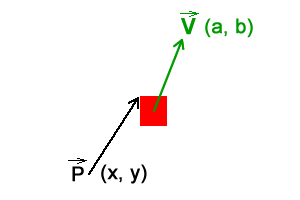
\includegraphics[scale = 0.5]{Bilder/pos_velocity_vectors.png}
\end{columns}
\end{frame}
\begin{frame}{Steering Behaviors (2)}
\begin{columns}
\column{0.5\textwidth}
\begin{itemize}
    \item Hinzunahme von angestrebter Geschwindigkeit
    \item Steuerungsvektor ist Resultat aus momentaner und angestrebter Geschwindigkeit
    \item Steuerung = Angestrebte Geschwindigkeit - Momentane Geschwindigkeit
\end{itemize}
\column{0.5\textwidth}
\begin{overprint}
\onslide<1>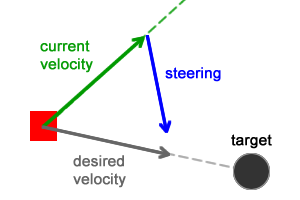
\includegraphics[scale = 0.5]{Bilder/steering_forces.png}
\onslide<2>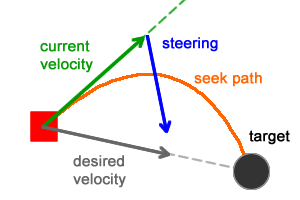
\includegraphics[scale = 0.5]{Bilder/steering_forces_seek_path.png}
\end{overprint}
\end{columns}
\end{frame}
\begin{frame}{Steering Behaviors (3)}
\begin{figure}

  \centering
  
  \begin{minipage}[b]{0.25\textwidth}
    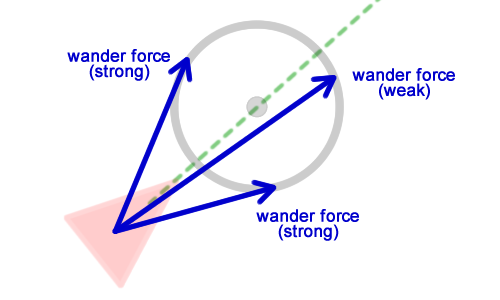
\includegraphics[scale = 0.2]{Bilder/wander_analyzing_wander_force.png}
    \caption{Wander}
  \end{minipage}
  \hfill
  \begin{minipage}[b]{0.25\textwidth}
    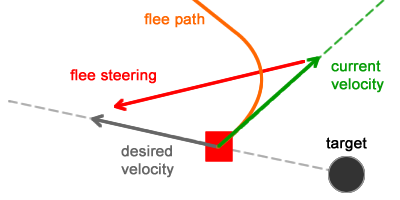
\includegraphics[scale = 0.2]{Bilder/steering_forces_flee_path.png}
    \caption{Flee}
  \end{minipage}
  \hfill
  \begin{minipage}[b]{0.25\textwidth}
    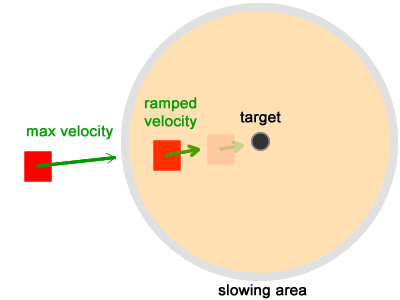
\includegraphics[scale = 0.2]{Bilder/steering_forces_arrival_velocities.png}
    \caption{Arrival}
  \end{minipage}
    
\end{figure}
\begin{figure}

  \centering
  
  \begin{minipage}[b]{0.25\textwidth}
    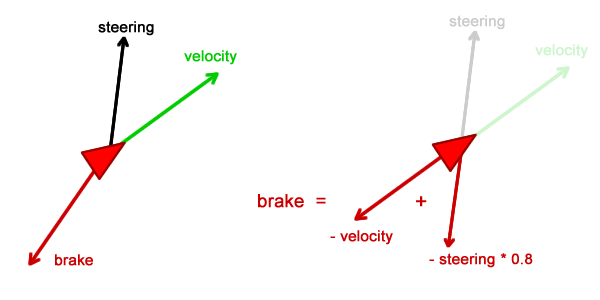
\includegraphics[scale = 0.2]{Bilder/queue_brake_force.png}
    \caption{Brake}
  \end{minipage}
  \hfill
  \begin{minipage}[b]{0.25\textwidth}
    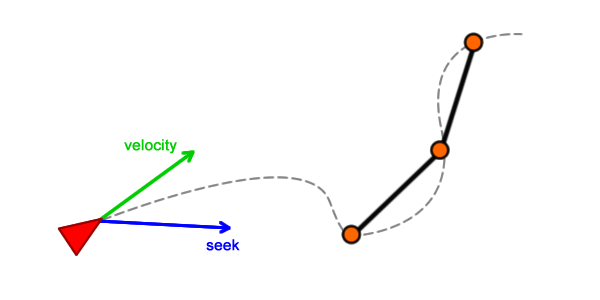
\includegraphics[scale = 0.2]{Bilder/path_seek_point.png}
    \caption{Path Following}
  \end{minipage}
  \hfill
  \begin{minipage}[b]{0.25\textwidth}
    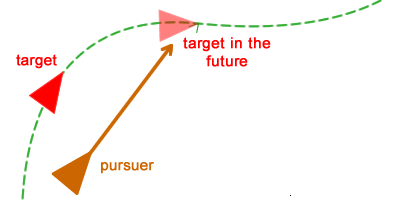
\includegraphics[scale = 0.2]{Bilder/pursuit_avoid_route.png}
    \caption{Pursuit}
  \end{minipage}
    
\end{figure}
\end{frame}
\begin{frame}{Dürfen wir vorstellen...?}
\begin{figure}

  \centering
  
  \begin{minipage}[b]{0.35\textwidth}
    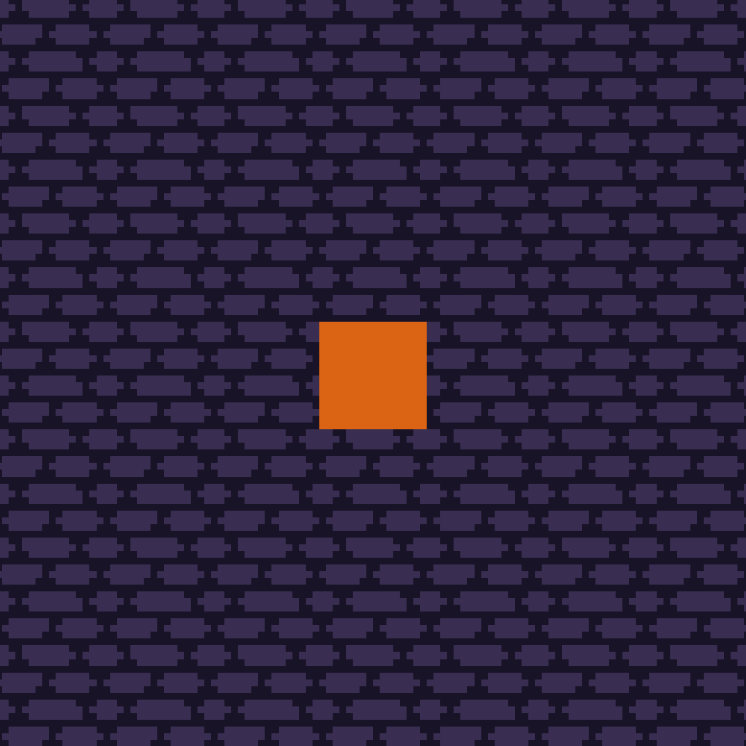
\includegraphics[scale = 0.2]{Bilder/WanderEnemy.png}
    \caption{Der Clotty (Wander)}
  \end{minipage}
  \hfill
  \begin{minipage}[b]{0.35\textwidth}
    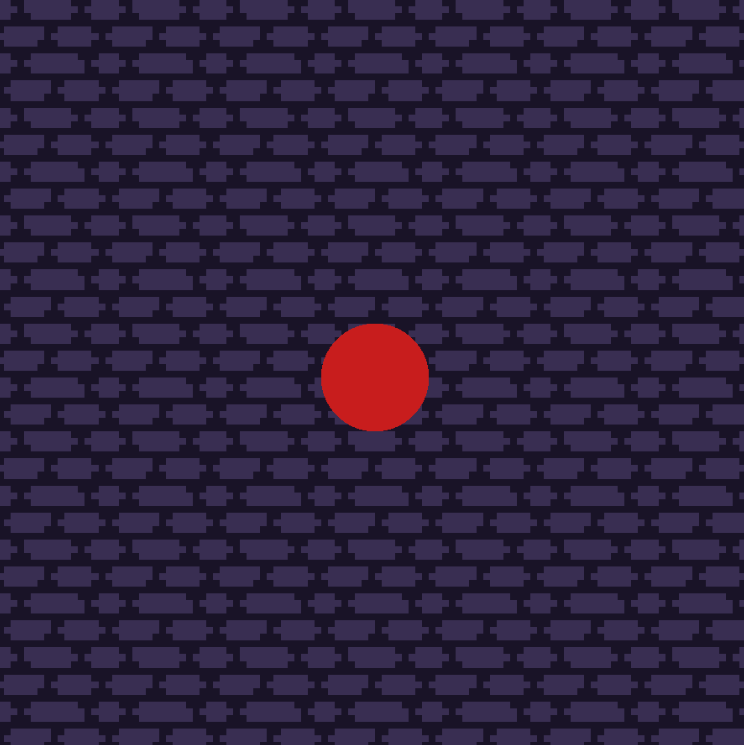
\includegraphics[scale = 0.2]{Bilder/MeleeEnemy.png}
    \caption{Der Globin (Seek)}
  \end{minipage}
    
\end{figure}
\end{frame}